\documentclass{article}
\usepackage[utf8]{inputenc}
\setlength{\parindent}{0em}
 \textwidth=6.5in
 \oddsidemargin=0pc
 \evensidemargin=0pc
 \topmargin=-2pc
 \headsep=0.05in
 \headheight=0pc
 \textheight=9.0in
 \setlength{\parskip}{2em}

\usepackage[shortlabels]{enumitem} 
\usepackage{array}
\usepackage{wrapfig}
\usepackage{multirow}
\usepackage{tabu}
\usepackage{comment}
\usepackage{amsmath}
\usepackage{algorithm}
\usepackage{algpseudocode}
\usepackage[table]{xcolor}
\usepackage{verbatim}
%this I used to draw a row major graph
\usepackage{tikz}
\newcommand\x{\times}
\newcommand\y{\cellcolor{olive!10}}
\usepackage{color,soul}
\newcommand{\hlc}[2][yellow]{ {\sethlcolor{#1} \hl{#2}} }



%how do you make roman numerals in the title ?? 
\title{Data Structure and algorithm II\\Homework 4}
\author{Jue,Guo}
\date{April 2019}

\begin{document}
\maketitle
Note: contain useful resources and reading material but not solution \\
Reference: \\
1. https://www.cs.princeton.edu/~wayne/kleinberg-tardos/pdf/05DivideAndConquerII.pdf \Comment{relationship between dot product and matrix multiplication}\\
2. https://www.purplemath.com/modules/inductn3.htm \Comment{Geometric series and its related math problem}\\
3. Introduction to Algorithms 3rd edition CH.27 \Comment{On the idea and concept of Parallel for}\\

\section{Recurrence and Time Complexity}
    At the first glance, this cannot be solved using master theorem. Since the f(n) here is $\Theta(\log ^{k} n)$, and our master theorem ask for $n^d$. So it does not conform.
    To fix it, we need to draw a recurrence tree of,
    
   \begin{equation*}
    T(n)=\left\{\begin{array}{l}{\theta(1) \text { if } \mathrm{n}=1} \\ {T\left(\frac{n}{2}\right)+\theta\left(\log ^{k} n\right) \quad \text { if } n>1}\end{array}\right.
    \end{equation*}
    
    This table contains the information of our recurrence tree:
  
    % this align the table content to the middle, sure better hope this works 
    \begin{tabu}  { | X[c] | X[c] | X[c] | X[c]|}
    \hline
        level&cost/problem&\# of nodes & cost/level \\
    \hline
        0&$\log ^{k} n$&1&$1(\log ^{k} n)$ \\
    \hline
        1&$\log ^{k} \frac{n}{2}$&1&$1*(\log ^{k} \frac{n}{2})$ \\
    \hline
        2&$\log ^{k} \frac{n}{4}$&1&$1*(\log ^{k} \frac{n}{4})$ \\
    \hline
        ...&...&...&... \\
    \hline 
        i&$\log ^{k} \frac{n}{2^i}$&1& $1*(\log ^{k} \frac{n}{2^i})$ \\
    \hline
         ...&...&...&... \\
    \hline
        n &$\log ^{k} \frac{n}{2^n}$&1& $1*(\log ^{k} \frac{n}{2^n})$ \\
    \hline
    
\end{tabu}
So, what is our "n"? It turns out that if we keep dividing our problems, we will end up of a problem size of 1. Solve for $\frac{n}{2^i}=1\ \text{and}\ n= \log_{2}n$. And the the worst case is:\ $\log n* \log^{k}n = \log^{k+1}n$.(Note: all level share the time complexity of $\log^{k}n$)\\
Now, we need to prove the best case scenario,$\Omega$,and one of the ideas I had is to expand out or some people like to say "unrolling" the  recurrence.
Let us take\ $n=2^m \ and \ m=logn$.Rewrite the recurrence:
%note to my self * is like reference symbol
\begin{equation*}
\begin{split}
T(n)&=T(2^m)\\&=T(\frac{2^m}{2})+\log^{k} 2^m\\
    &=T(2^{m-1})+ (m\log2)^k\\&=T(2^{m-1})+ (m)^k\\
    \end{split}\end{equation*}

This looks a bit messy too, so lets simplify it further, letting $T(2^m)=f(m)$\\
Rewrite:
\begin{equation*}
\begin{split}
f(m)&=f(m-1)+m^k\\&=f(m-2)+(m-1)^k+m^k\\
    &=f(m-3)+(m-2)^k+(m-1)^k+m^k\\
    &=f(m-4)+(m-3)^k+(m-2)^k+(m-1)^k+m^k\\
    &=f(0)+...+f(m-4)+(m-3)^k+(m-2)^k+(m-1)^k+m^k\\
    \end{split}\end{equation*}
\text{Note: $n=2^m$,and that is why we went all the way to $f(0)$} \\
To be honest: we can also use this to prove our $O$, but I am late to the party,so...\\
Let's prove lower bound \ $\Omega$, like a computer scientist or a mathematician, let's write it out in English, so everyone knows what is going on here;\ 
We now have:
\begin{equation*}
\begin{split}
 f(m)&=f(0)+...+f(m-4)+(m-3)^k+(m-2)^k+(m-1)^k+m^k\\
        &=f(0)+1^k+2^k+3^k+.....+m^k \\
    \end{split}\end{equation*}
Now we simply need to prove the $\Omega$ of $1^k+2^k+3^k+.....+m^k$.        
And, we can prove this by "throwing away half of the item"
\begin{equation*}
    \begin{split}
1^k+2^k+3^k+.....+m^k &> (\frac{m}{2})^k+ (\frac{m}{2}+1)^k +...+m^k\\ 
                     &>\underbrace{\left(\frac{m}{2}\right)^{k}+\left(\frac{m}{2}\right)^{k}+\ldots+\left(\frac{m}{2}\right)^{k}}_{\frac{m}{2} \text { terms }}\\
                     &=\frac{m}{2}\left(\frac{m}{2}\right)^{k}\\
                     &=(\frac{m}{2})^{k+1}\\
    \end{split}
\end{equation*}

Therefore,$f(m)=\Omega(m^{k+1})$,because $f(m)>c*(m^{k+1})$ and $c=\frac{1}{2^{k+1}}$\\
In other word, our $T(n)=\Omega(log^{k+1}n)$.We already proved our worst case using recursion tree $T(n)=O(log^{k+1}n)$,So we have $T(n)=\Theta(log^{k+1}n)$. 
 \newpage
\section{Matrix Multiplication}
\begin{enumerate}[(a)] % (a), (b), (c), ...

\item Time complexity of parallel dot product

\begin{center}
\algrenewcommand\textproc{}
\begin{algorithm}
\renewcommand{\thealgorithm}{2.a):}
\caption{Multi-thread Dot product}
\begin{algorithmic}[1]

    \Function{d=PAR-DOT-PROD}{x,y} 
\If{length(x)=1}
\State \textbf{return} $x\cdot y$
   % \\ \Return $\vars{x\cdot y}$
\EndIf
\State split $x =[x_L\ x_R]$ and $y=[y_L\  y_R]$
\State\textbf{spawn} $d_L=$ PAR-DOT-PROD$(x_L,y_L)$
\State$d_R=$ PAR-DOT-PROD$(x_R,y_R)$
\State\textbf{sync}
\State\textbf{return} $d_L + d_R$
\EndFunction
\end{algorithmic}
\end{algorithm}
\end{center}
To solve work,$T_1$,we need to cover up the spawn part of the code:
\begin{center}
   \textbf{spawn} $d_L=$ PAR-DOT-PROD$(x_L,y_L)$\\
   \textbf{spawn} $d_R=$ PAR-DOT-PROD$(x_R,y_R)$\\
\end{center}
So,what I see is it is doing 2 recursive calls, and the problem size is divided into 2 parts. So our a=2 and our b=2 in our recursive function,\ $T_1=2T(\frac{n}{2})+O(1)$ and our span is: $T_\infty=T(\frac{n}{2})+O(1)$. \\
Looks like we can use Master Theorem to solve this and get time complexity of this recurrence: 

%This block is master theorem. Reuse-able. 
$\text {Master theorem} \text { If } T(n)=a T(\lceil n / b\rceil)+O\left(n^{d}\right) \text { for some constants } a>0, b>1, \text { and } d \geq 0$ \text{,then}
\begin{equation*}
T(n)=\left\{\begin{array}{ll}{O\left(n^{d}\right)} & {\text { if } d>\log _{b} a\text{\ $\cdot \cdot \cdot $ case 1}} \\ {O\left(n^{d} \log n\right)} & {\text { if } d=\log _{b} a\text{\ $\cdot \cdot \cdot$ case 2}} \\ {O\left(n^{\log _{b} a}\right)} & {\text { if } d<\log _{b} a\text{\ $\cdot \cdot \cdot $ case 3}}\end{array}\right.
\end{equation*}\\
Therefore, \\
1.$T_1(n)=2T(\frac{n}{2})+O(1)$ has $a=2,b=2,d=0$,so $\log_{2}2=1>d=0$ and this is case 3 of master theorem: $T_1={O(n^{\log_{2}2})=O(n)}$. \\
2.$T_\infty(n)=T(\frac{n}{2})+O(1)$ has $a=1,b=2,d=0$,so $\log_{2}1=0=d=0$ and this is case 2 of master theorem: $T_\infty=O(n^0\log n)=O(\log n)$
\newpage
\item Use parallel dot product as subroutine\\
To figure out the algorithm, we try go back all the way to the understanding of the the basic idea of the dot product and its relationship with the matrix multiplication. 

\begin{equation*}
c=a \cdot b = \sum_{i=1}^{n} a_{i} b_{i}
\end{equation*}

This might seem too abstract, so lets use example to help us:\footnote{"L" and "R" refer to Algorithm:2.a)} 
\begin{equation*}
\begin{split}
a&=\left[\begin{array}{lll}{.70} & {.20} & {.10}\end{array}\right]\\
b&=\left[\begin{array}{lll}{.30} & {.40} & {.30}\end{array}\right]\\
a\cdot b&=\underbrace{(.70 \times .30)}_{L}+(.20 \times .40)+\underbrace{(.10 \times .30)}_{R}=.32\\
\end{split}
\end {equation*}
And how does dot product help us with the matrix multiplication:
For example if we have $n\times n$ matrix A,B,C and let C=AB and for me cause I like to think what looks like when I actually write in code: what is the right value to fill in my matrix C. 
\begin{equation}
c_{i j}=\sum_{k=1}^{n} a_{i k} b_{k j}
\end{equation}
Visually,
%n by n matrix multiplication reusable
\begin{equation*}\left[ \begin{array}{cccc}{c_{11}} & {c_{12}} & {\cdots} & {c_{1 n}} \\ {c_{21}} & {c_{22}} & {\cdots} & {c_{2 n}} \\ {\vdots} & {\vdots} & {\ddots} & {\vdots} \\ {c_{n 1}} & {c_{n 2}} & {\cdots} & {c_{n n}}\end{array}\right]=\left[ \begin{array}{cccc}{a_{11}} & {a_{12}} & {\cdots} & {a_{1 n}} \\ {a_{21}} & {a_{22}} & {\cdots} & {a_{2 n}} \\ {\vdots} & {\vdots} & {\ddots} & {\vdots} \\ {a_{n 1}} & {a_{n 2}} & {\cdots} & {a_{n n}}\end{array}\right] \times \left[ \begin{array}{cccc}{b_{11}} & {b_{12}} & {\cdots} & {b_{1 n}} \\ {b_{21}} & {b_{22}} & {\cdots} & {b_{2 n}} \\ {\vdots} & {\vdots} & {\ddots} & {\vdots} \\ {b_{n 1}} & {b_{n 2}} & {\cdots} & {b_{n n}}\end{array}\right]\end{equation*}
What looks using an example:
%this is how you highlight a column
\begin{equation*}
    \left[ \begin{array}{ccc}
    .59 & \y.32 & .41 \\ 
    .31 & .36 & .25 \\ 
    .45 & .31 & .42\end{array}\right]
    =
    \left[ \begin{array}{ccc}
     \rowcolor{olive!20}
    .70 & .20 & .10 \\ 
    {.30} & {.60} & {.10} \\ 
    {.50} & {.10} & {.40}
    \end{array}\right]
    \times
    \left[ \begin{array}{c>{\columncolor{olive!20}}cc}
    {.80} & {.30} & {.50} \\ 
    {.10} & {.40} & {.10} \\ 
    {.10} & {.30} & {.40}
    \end{array}\right]
\end{equation*}

%block comment(Later I gave it some thought and do not think this is useful BUT keeping it because it is row major graph and it is fun)
\begin{comment}
I think I will use row major for my algorithm:
\begin{center}
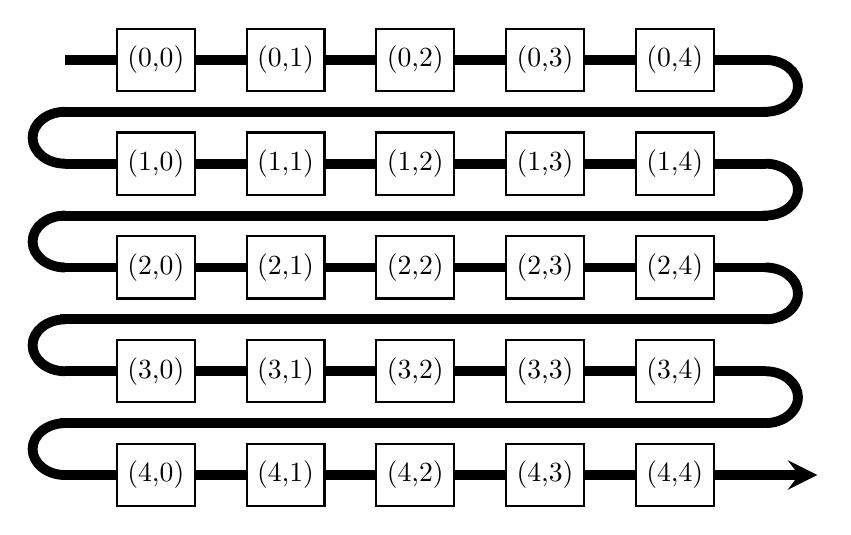
\begin{tikzpicture}[>=stealth,x=0.75pt,y=0.75pt,yscale=-1,xscale=1.25,color=black,line width=1.25mm, opacity=1]
%xscale = 1.25 will increase horizontal size and spacing
%yscale with a negative sign makes the (0,0) at the top right corner

%boxes with numbers
 \foreach \x in  {0,...,4}
    \foreach \y in  {0,...,4 }
     \foreach \position in {(50*\x,50*\y)}
            { \draw[thick] \position rectangle +(30,30) node[pos=0.5] {(\y,\x)} ;}

%lines through the boxes
\tikzstyle{arrow} = [->,>=stealth,color=black,line width=1.25mm, opacity=1]
\foreach \x in {0,...,5}
\foreach \y in {0,...,4}
{\draw  (-20+50*\x,15+50*\y) -- (00+50*\x,15+50*\y);
}
\draw[arrow] (230,215) -- (270,215);  %arrow head at box (4,4)

%arcs at the end
\foreach \y in {0,...,3}
{\draw  (250,15+50*\y) arc(270:455:12.5); 
\draw (-20,65+50*\y) arc(90:270:12.5);
\draw (-22,40+50*\y) -- (251, 40+50*\y);
}
\end{tikzpicture}
\end{center}
\end{comment}

%some new ideas 
%Algorithm 2.b)
Referring to the idea from above and let's write out the algorithm:
\algrenewcommand\textproc{}
\begin{algorithm}
\renewcommand{\thealgorithm}{2.b):}
\caption{Matrix Multiplication}\Comment{$c_{i j}=\sum_{k=1}^{n} a_{i k} b_{k j}$}\\
\textbf{Input}: $n\times n$ Matrix A and B \\
\textbf{Output}: $n\times n$ Matrix C
\begin{algorithmic}[1]
\Function{PAR-MATMUL}{A,B} 
\State $k= $A.row  \Comment{$\sum_{k=1}^{n} $}\\
\   \ \textbf{para for} i=0 to k 
\State\textbf{para for} j=0 to k 
\State $c_{ij}=$PAR-DOT-PROD($A_{ik},B_{kj}$) \\
\Comment{$a_{i k} b_{k j}$ \&$A_{ik}$,$B_{kj}$ represent corresponding row of A and and column of B like marked gray as above } \\
\ \ \textbf{end para for}
\State\Return C
\EndFunction
\end{algorithmic}
\end{algorithm}
\newpage
Complexity Analysis of \textbf{2.b)}: \\
If I remember correctly from class:
A compiler can implement each parallel for loop as a divide-and-conquer subroutine using nested parallelism.Cover up the \textbf{para for} when finding the work:

$T_{1}(n)$= $n*n*T^{'}_1(n)$, and$ T^{'}_1(n)$ represent the work of PAR-DOT-PROD(), so we have $T_{1}(n)$=$O(n^3)$

To find the span: the inner \textbf{parallel for} has complexity of 
$O(\log n)$ and it dominate the constant time work of each iteration and the logic apply to outer \textbf{parallel for} as well. So,
$T_{\infty}(n)$=$O(\log{n})$



\end{enumerate}
\section{All-Pairs Shortest Paths}

\algrenewcommand\textproc{}
\begin{algorithm}
\renewcommand{\thealgorithm}{3:}
\caption{All-Pairs Shortest Paths}
\begin{algorithmic}[1]
\Function{C = APSP}{A} 
\If {dimension(A) = 1}
\State \textbf{return} 0
\EndIf 
\State partition A=$\left[ \begin{array}{ll}{A_{11}} & {A_{12}} \\ {A_{21}} & {A_{22}}\end{array}\right]$and C= $\left[ \begin{array}{ll}{C_{11}} & {C_{12}}\\ {C_{21}} & {C_{22}}\end{array}\right]$
into equal-sized quadrants
\State \hlc[red]{C11 = APSP(A11)}
\State \hl{\textbf{spawn} A12 = par-trop-matmul(A11, A12)}
\State \hl{A = par-trop-matmul(A21, A11}
\State \textbf{sync}
\State \hl{$A_{22}$= min\{$A_{22}$, par-trop-matmul($A_{21}, A_{12}$)\} }
\State \hlc[red]{$C_{22}$ = APSP($A_{22}$)}
\State \hl{\textbf{spawn} $A_{12}$ = par-trop-matmul($A_{12}$, $A_{22}$)}
\State \hl{$A_{21} = \text{par-trop-matmul}(A_{22}, A_{21})$}
\State \textbf{sync}
\State \hl{$A_{11} = min\{A_{11},\text{par-trop-matmul} (A_{12}, A_{21})\}$}
\State \textbf{return} C
\EndFunction
\end{algorithmic}
\end{algorithm}

After talking with professor Ballard about the question, I think I have an idea of how to do this. I learned that  $A_{22}$= $min$\{$A_{22}$, par-trop-matmul($A_{21}, A_{12}$)\} and $min\{A_{11},\text{par-trop-matmul} (A_{12}, A_{21})\}$
are like $C+AB$ and we can see this of having the same time complexity as our PAR-MATUAL. So,our work will be
\begin{equation*}
\begin{split}
  T_{\infty}(n)&=\underbrace{2T_1(\frac{n}{2})}_{APSP}+\underbrace{6P((\frac{n}{2}))}_{par-trop-matmul}\\
  &=2T_1(\frac{n}{2})+6*O((\frac{n}{2})^3) \ \  \text{Note: Ignore constant $\frac{6}{8}$}\\
  &=2T_1(\frac{n}{2})+O(n^3) \end{split}\end{equation*}
  

Looks like we can apply master theorem: $a=2, b=2,\text{and}\ d=3$ and our $\log_{2}2 =1$, which $d=3>1$ meaning case 1 of master theorem applies and $ T_{1}(n)=O(n^3).$ 

Span: \begin{equation*}
\begin{split}
  T_{\infty}(n)&=\underbrace{2T_1(\frac{n}{2})}_{APSP}+\underbrace{4P((\frac{n}{2}))}_{par-trop-matmul}\\
  &=2T_1(\frac{n}{2})+4*O(\log\frac{n}{2}) \ \  \text{Note: Ignore constant $4$ and $\log2=1$}\\
  &=2T_1(\frac{n}{2})+O(\log n) \end{split}\end{equation*}
  
Looks like master theorem is a no go. So let's use our dear old friend recurrence tree: 

\begin{tabu}  { | X[c] | X[c] | X[c] | X[c]|}
    \hline
        level&cost/problem&\# of nodes & cost/level \\
    \hline
        0    &$\log ^{k} n$&1&$1(\log ^{k} n)$ \\
    \hline
        1&$\log ^{k} \frac{n}{2}$&2&$2*(\log ^{k} \frac{n}{2})$ \\
    \hline
        ...&...&...&... \\
    \hline 
        i&$\log ^{k} \frac{n}{2^i}$& $2^i$ & $2^i*(\log ^{k} \frac{n}{2^i})$ \\
    \hline
         ...&...&...&... \\
    \hline
        $L=\log_{2}n$ &$1$& $2^L$ & n  \\
    \hline
    
\end{tabu}

OK,this is math. We need to do it no matter what! Let's add cost of each level up. Are you excited? If you start grading from top to bottom, probably not, but I am. We did this prove on $M_1$ of parallel merge sort, but I will clarify and format it. 
\begin{equation*}
    \begin{split}
       T_\infty(n)&=\underbrace{\log _{2} n+2 \log _{2}\left(\frac{n}{2}\right)+4 \log _{2}\left(\frac{n}{4}\right)+8 \log _{2}\left(\frac{n}{8}\right)+\ldots}_{\log _{2} n \operatorname{tines}}\\
       &=\sum_{i=0}^{\log_{2}n} 2^i \log (\frac{n}{2^i})\\
       &=\sum_{i=0}^{\log _{2} n} 2^{i}\left(\log n-\log 2^{i}\right)\\
       &=\sum_{i=0}^{\log _{2} n} 2^{i} \log n-\sum_{i=0}^{\log _{2} n} 2^{i} \log 2^{i}\\
       &=\sum_{i=0}^{\log _{2} n} 2^{i} \log n -\sum_{i=0}^{\log _{2} n} i \cdot 2^{i}\\
       &=\log n\sum_{i=0}^{\log _{2} n} 2^{i}-\sum_{i=0}^{\log _{2} n} i \cdot 2^{i}
       \ \rightarrow\text{Geometric series:$
\sum_{i=1}^{n} a_{1} r^{i-1}=S_{n}=\frac{a_{1}\left(1-r^{n}\right)}{1-r} , r \neq 1
$}\\
       &= \log n \sum_{i=0}^{\log _{2} n}\left(2^{i-1}\right) \cdot 2-\sum_{i=0}^{\log _{2} n} i \cdot 2^{i}\\
       &= -2\log n +2n -\sum_{i=0}^{\log _{2} n} i \cdot 2^{i} \ \rightarrow\text{refer to James Stewart Calculus$\sum_{k=1}^{n} k 2^{k}=2\left(2^{n} n-2^{n}+1\right)$}\\
       &=-2\log n +2n-2 \cdot\left(2^{\log _{2} n} \cdot \log _{2} n-2^{\log _{2} n}+1\right)\\
       &=-2\log n +2n-2( n \log n-n+1)\\
       &=2\log n -2n\log n +4n -2 \\
       &=O(n)\\
    \end{split}
\end{equation*}
 
    
\end{document}